\documentclass{article}
\usepackage{graphicx} % Required for inserting images

\title{Final Assignment\\[0.2cm]Computer Workshop}
\author{amirmohammad iranmanesh}
\date{January 2025}



\begin{document}

\maketitle
\newpage
\section{Git and GitHub}
    \subsection{Repository Initialization and Commits}
    first of all, I created a new repository by selecting new repository from the up-left the plus section.
    \\ second I copied the https link of the repository from the code section I cloned it to my PC by command: \texttt{git clone \textless https link of repository\textgreater}.
    \subsection{GitHub Actions for LaTeX Compilation}
     first i made this directory ".github/workflows" in my repository folder. I created this file "latex-build.yml" in workflows folder, and then I copied the text from the link inside the pdf in "latex-build.yml". and changed the main.tex to the name of my file "The Final Assignment", but it wasn't enough. In github i saw an error that was related to some permission, so i added this "permissions: write-all" to  "latex-build.yml".

\section{Exploration Tasks}
    \subsection{Vim Advanced Features}
    \begin{enumerate}
        \item Access multiple named and unnamed registers for copy-pasting and storing text.
        \item Vim supports multiple windows and buffers, allowing you to work on multiple files or sections simultaneously.
        \item Vimscript allows you to create custom scripts to extend Vim's functionality.
    \end{enumerate}
    \subsection{Memory profiling}
        \subsubsection{Memory Leak}
        A memory leak occurs in a program when it allocates memory dynamically (using malloc or calloc in C) but fails to free it after it's no longer needed. This causes the allocated memory to remain unusable until the program terminates, which can lead to increased memory consumption and eventual system performance issues.
        \\\textbf{how they happen:}
        \begin{enumerate}
            \item \textbf{Failure to Free Memory:} Forgetting to call free() for dynamically allocated memory.
            \item \textbf{Lost References:} Overwriting or losing the pointer to the allocated memory without freeing it.
            \item \textbf{Improper Pointer Management:} Freeing memory and then continuing to use the dangling pointer.
            \item \textbf{Loops or Recursions:} Repeated allocations in loops or recursive functions without freeing memory in each iteration.
        \end{enumerate}
        \subsubsection{Memory profilers}
        Valgrind provides a suite of tools to:
        \begin{enumerate}
            \item Detect memory management errors (leaks, invalid memory access).
            \item Check for uninitialized memory usage.
            \item Identify threading issues (race conditions).
        \end{enumerate}
        Valgrind tracks all memory allocations and deallocations in a program. If memory is allocated but not freed before the program terminates, it flags this as a memory leak.
        \\This command \textbf{"valgrind --leak-check=full ./yourprogram"} will run your program under Valgrind, and it will display a detailed report of any memory leaks or issues detected.
    \subsection{GNU/Linux Bash Scripting}
        \subsubsection{fzf}
        \begin{itemize}
            \item Fuzzy searching is a technique that locates items in a dataset that approximately match a given pattern, even when there are minor discrepancies or errors.
            \item The command \texttt{(ls | fzf)} lists the files and directories in the current folder (\texttt{ls}) and passes them to (\texttt{fzf}). It lets you search and select items from the list using approximate matching. when you select an item, its name is printed to the terminal.
        \end{itemize}
        \subsubsection{Using fzf to find your favorite PDF}
        \begin{enumerate}
            \item this command \texttt{(fd -e pdf)} will list all files with the .PDF extension
            \item when we have the list of .PDF files, we can send the output to fzf to select a PDF from the data gathered. that’s the command: \texttt{fd -e pdf | fzf}
        \end{enumerate}
        \subsubsection{Opening the file using Zathura}
        To open the selected PDF using Zathura, use this command:\\ 
        \texttt{zathura "\$(fd -e pdf | fzf)"}.
        \\\texttt{fd -e pdf} lists all files with the .pdf extension. \texttt{| fzf} sends the list to fzf. \texttt{zathura "\$( ... )"} 
         opens the selected file with Zathura. The \texttt{\$( ... )} syntax captures the selected file path and passes it to Zathura.

\section{Git and FOSS}
    \subsection{README.md}
    \subsection{Issues}
    \begin{figure}[h]
    \centering
    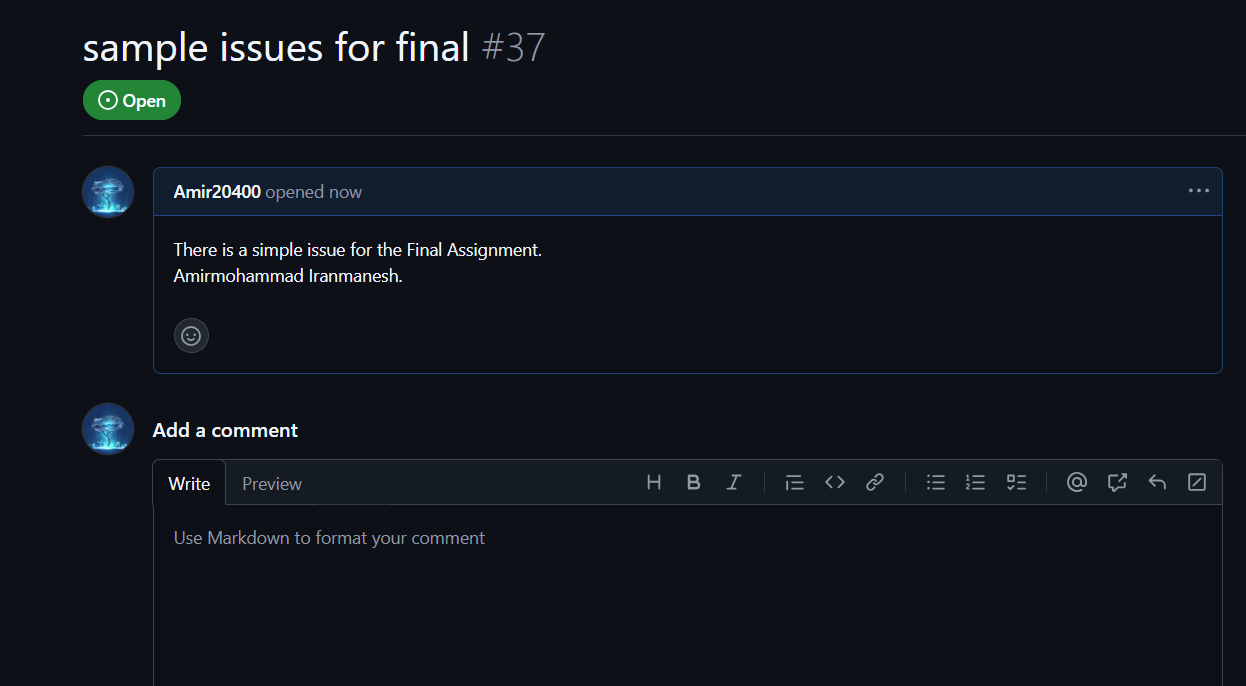
\includegraphics[width=0.8\textwidth]{sample issue.png}
    \caption{sample issue}
    \end{figure}
        
\end{document}
